%!TeX root=./cinetico.tex

\FloatBarrier
\subsection{Tratamento de casos degenerados}

Como citado anteriormente, a nossa fila de prioridade $Q$ guarda os
certificados cuja chave é $t$, o instante de tempo em que o
certificado expira. Porém, é possível que dois ou mais certificados
expirem no mesmo instante de tempo $t$, configurando um empate na
nossa fila. Nos problemas anteriores, tais empates costumavam ser
tratados por algum critério de desempate que era suficiente para
garantir que as estruturas permanecessem corretas. No entanto, para
o par mais próximo cinético encontrar tal critério não é uma tarefa
tão simples.

Para olhar mais profundamente para o problema vamos antes considerar
que os eventos associados ao torneio não fazem parte da fila.

Algumas situações em que dois certificados vencem no mesmo instante
acabam não causando problemas, por exemplo, dois eventos que
envolvem pares de pontos distintos $(p, q)$ e $(r, s)$, ocorrendo no
mesmo instante de tempo $t$. Contudo, quando dois pontos se colidem,
isto é, atingem a mesma posição em $\real^2$ num instante $t'$,
ocorrem trocas nas três direções ($0^\circ$, $+60^\circ$ e
$-60^\circ$). Essas trocas precisam ser realizadas de maneira
consistente, para que as estruturas possam ser atualizadas da devida
maneira.

% Melhorar esse parágrafo
A colisão não necessariamente envolve apenas dois pontos, podem
haver mais pontos se colidindo no mesmo instante e, nesse caso,
precisamos nos preocupar também como as trocas afetam os pares de
pontos, mas como elas afetam todos o pontos envolvidos no geral.

Para determinar em que ordem os eventos devem ocorrer podemos
simular um evento não degenerado. No caso, vamos simular que os
pontos desviam em uma trajetória circular, ao longo de uma
circunferência de raio proporcional à sua velocidade, com mesma
velocidade angular, e depois seguem em frente normalmente em suas
trajetórias lineares. Adicionaremos então um parâmetro $\theta \in
[0, \pi]$ que indica o ângulo a ser percorrido até que o evento
aconteça simulando essa trajetória circular, veja a figura
\ref{degen:exemplo}.

\begin{figure}[H]
    \centering
    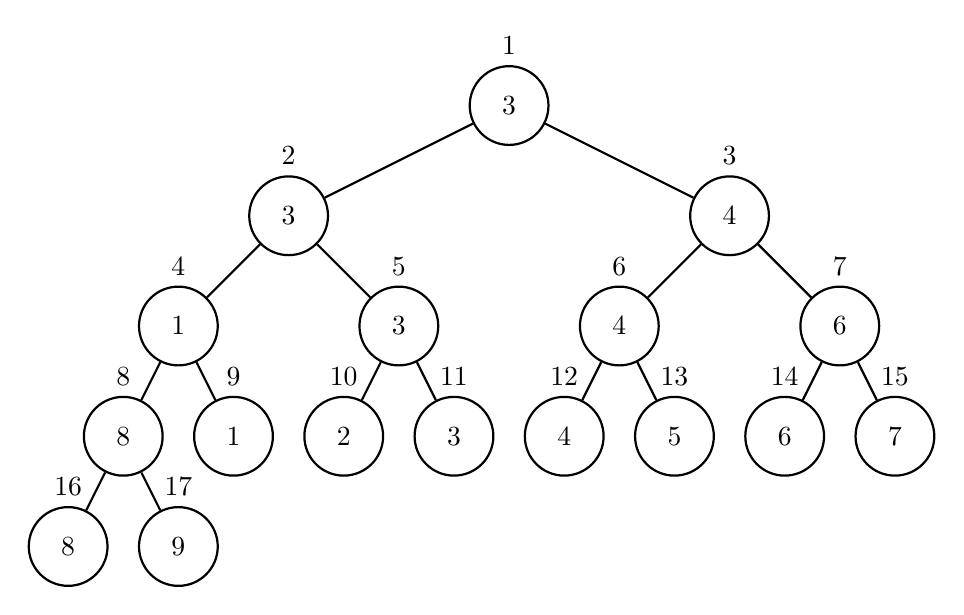
\begin{tikzpicture}[thick, scale=0.7]
        \node[label={1},circle,draw,minimum size=1cm]
        (1) at (0,0) {$3$};
        \node[label={2},circle,draw,minimum size=1cm]
        (2) at (-4,-2) {$3$};
        \node[label={3},circle,draw,minimum size=1cm]
        (3) at (4,-2) {$4$};
        \node[label={4},circle,draw,minimum size=1cm]
        (4) at (-6,-4) {$1$};
        \node[label={5},circle,draw,minimum size=1cm]
        (5) at (-2,-4) {$3$};
        \node[label={6},circle,draw,minimum size=1cm]
        (6) at (2,-4) {$4$};
        \node[label={7},circle,draw,minimum size=1cm]
        (7) at (6,-4) {$6$};
        \node[label={8},circle,draw,minimum size=1cm]
        (8) at (-7,-6) {$8$};
        \node[label={9},circle,draw,minimum size=1cm]
        (9) at (-5,-6) {$1$};
        \node[label={10},circle,draw,minimum size=1cm]
        (10) at (-3,-6) {$2$};
        \node[label={11},circle,draw,minimum size=1cm]
        (11) at (-1,-6) {$3$};
        \node[label={12},circle,draw,minimum size=1cm]
        (12) at (1,-6) {$4$};
        \node[label={13},circle,draw,minimum size=1cm]
        (13) at (3,-6) {$5$};
        \node[label={14},circle,draw,minimum size=1cm]
        (14) at (5,-6) {$6$};
        \node[label={15},circle,draw,minimum size=1cm]
        (15) at (7,-6) {$7$};
        \node[label={16},circle,draw,minimum size=1cm]
        (16) at (-8,-8) {$8$};
        \node[label={17},circle,draw,minimum size=1cm]
        (17) at (-6,-8) {$9$};

        \draw[thick] (1) -- (2);
        \draw[thick] (2) -- (4);
        \draw[thick] (4) -- (8);
        \draw[thick] (4) -- (9);
        \draw[thick] (8) -- (16);
        \draw[thick] (8) -- (17);
        \draw[thick] (2) -- (5);
        \draw[thick] (5) -- (10);
        \draw[thick] (5) -- (11);
        \draw[thick] (1) -- (3);
        \draw[thick] (3) -- (6);
        \draw[thick] (3) -- (7);
        \draw[thick] (6) -- (12);
        \draw[thick] (6) -- (13);
        \draw[thick] (7) -- (14);
        \draw[thick] (7) -- (15);
    \end{tikzpicture}
    \caption[Representação da estrutura torneio]{Torneio com $9$
        elementos em que $3$ é o elemento com valor máximo.}
    \label{fig:torneio:exemplo}
\end{figure}

Como esse novo critério de desempate somos capazes de simular essa
trajetória não degenerada e os eventos ocorrerão em uma ordem
apropriada, veja um exemplo na figura \ref{degen:exemploeventos}.

\begin{figure}
    \centering
    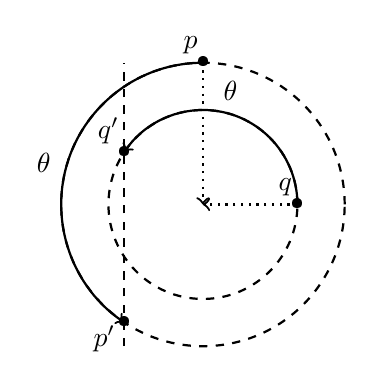
\begin{tikzpicture}[thick, scale=0.6]
        \node[label={[label distance = -3mm]160:$p$}] at
            (0, 3) {\textbullet};
        \node[label={[label distance = -3mm]160:$q$}] at
            (2, 0) {\textbullet};

        \draw[->, dotted] (0, 3) -- (0, 0); % p arrow
        \draw[->, dotted] (2, 0) -- (0, 0); % q arrow

        \draw[dashed] (0,0) circle[radius=3];
        \draw[dashed] (0,0) circle[radius=2];

        \draw[->] (0, 3) arc(90:236:3) node[midway, xshift=-3mm] {$\theta$};
        \draw[->] (2, 0) arc(0:146:2) node[midway, yshift=3mm] {$\theta$};
        \node[label={[label distance = -3mm]160:$q'$}] at
            (-1.6634, 1.1104) {\textbullet};
        \node[label={[label distance = -3mm]260:$p'$}] at
            (-1.6634, -2.4952) {\textbullet};

        \draw[dashed] (-1.664, -3) -- (-1.664, 3); % p arrow
    \end{tikzpicture}
    \caption{Exemplo de parâmetro de evento horizontal ocorrendo
    entre $p$ e $q$, com a trajetória simulada.}
    \label{degen:exemploeventos}
\end{figure}

Existe ainda um outro detalhe de implementação que vale ser
mencionado: quando temos vários pontos se colidindo no mesmo
instante $t'$ diversos eventos serão acionados em uma determinada
ordem e, durante as alterações realizadas nos eventos, são
realizadas checagens de predecessor e sucessor em uma determinada
ordem. Porém, se os dois pontos se encontram na exata mesma posição,
não é possível determinar quem é o sucessor e quem é o predecessor
considerando apenas a posição dos pontos.

Um critério que pode ser utilizado para resolver esse problema é o
seguinte: se os dois pontos possuem a mesma coordenada é certo que
existiu, existe ou existirá um certificado na fila relacionado à
troca da ordem entre eles em uma determinada direção. Então,
comparamos esse certificado com o certificado atual da fila para
verificar se ele já foi processado ou ainda virá a ser processado.
Com isso, podemos determinar se queremos saber da situação em um
instante $t' - \epsilon$ ou $t' + \epsilon$, que pode ser computada
facilmente considerando apenas o vetor velocidade dos pontos.
